\newpage
\subsection{Tuning Deep Neural Architectures with Genetic Algorithm}
\label{sec:tuning_deep_nets_with_ga}
Training deep neural networks especially determining good hyperparameters is difficult, traditionally the hyperparameters of the network is based on human intuition alone, however having discovered \cite{kitano1990empirical, leung2003tuning, montana1989training}
, we hypothesize perhaps there is some value in automatically tuning the hyperparameters of a deep neural network by using a Genetic Algorithm.

Genetic Algorithms (GA) are meta-heuristics inspired by biological evolution, used to find global optimal solutions with genetic operators such as selection, crossover and mutation (see Algorithm~\ref{al:ga})~\cite{john1992adaptation, mitchell1998introduction}. 

\begin{wrapfigure}{L}[0pt]{0.48\textwidth}
	\vspace{-0.8cm}
	\begin{minipage}[t]{0.48\textwidth}
		\begin{algorithm}[H]
			\caption{Genetic Algorithm}
			\label{al:ga}
			
			\begin{algorithmic}
				\STATE{Let $P$ be the Population}
				\STATE{Let $I$ be an Individual in the Population} 
			    \STATE
				\STATE{Initialize population}
				\STATE
				\WHILE{True}
					\STATE{Evaluate $P$}
					\STATE
					\IF{$I \in P$ satisfies termination critera}
						\STATE{Break loop}
					\ENDIF	
					\STATE
					\STATE{Select Parents}
					\STATE{Crossover Offspring}
					\STATE{Mutate Offspring}
				\ENDWHILE
			\end{algorithmic}
		\end{algorithm}
	\end{minipage}
	\vspace{-0.4cm}
\end{wrapfigure}

The algorithm begins by initializing a random population where individuals are representations of a potential solution, then each individual is evaluated with an evaluation function, at this point if an individual within the population satisfies a termination criteria (e.g.\ fitness or generation) the algorithm is terminated, else the algorithm continues. The first genetic operator is the selection operator where individuals with better fitness scores are biased in being selected to become parents to reproduce off-springs. The off-springs are then subjected to the crossover and mutation genetic operators that encourage their genomes to diversify and converge to a better solution. This process is repeated from the point where the population is evaluated until a termination criteria is reached. For more information on how the genetic operators work see supplementary material \ref{sup:genetic_operators}.



\subsubsection{Preliminary Experiments and Results}

\begin{wrapfigure}{R}[0pt]{0.3\textwidth}
	\vspace{-0.4cm}
	\centering
	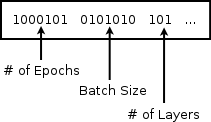
\includegraphics[width=0.25\textwidth]{sections/imgs/ga/ga_encoding.png}
	\caption{Problem Encoding}
	\label{fig:ga_encoding}
\end{wrapfigure}

We used the MNIST~\cite{lecun1998mnist} dataset of handwritten digits to test the idea of using GA to tune a feed-forward network and compared it with Random Walk (RW), for our purpose and time contraints \textbf{only 10\% of the dataset was used} for the experiment. The hyperparameters tuned in both approaches include the number of epochs, batch size, number of layers, number of hidden neurons at each layer, the activation functions, dropout rates at each layer as well as the optimizer used (e.g. SGD, Ada Delta, RMS back-propagation, etc). 

For this experiment the GA approach was inspired by \cite{whitley1990genetic} and we used a similar direct-encoding representation of the hyperparameters with a bit string (see Fig~\ref{fig:ga_encoding}). We used tournament selection, point crossover and multiple point mutation as the genetic operators, the following parameters were used generation limit of 20, population size 10, tournament selection size 2, crossover probability 50\%, mutation probability 80\%, mutation percentage 10\% (i.e. 10\% of the chromosome will be mutated). With RW the configuration is very similiar except a max iteration of 200 ($20~\text{individuals} \times 10~\text{generations}$), population of size 1, but the absents of both selection and crossover genetic operators. Both used a fitness function based on the classification accuracy (0 to 1.0) of the network using the test dataset.


\begin{figure}[H]
	\centering
	\begin{subfigure}[b]{0.45\linewidth}
	    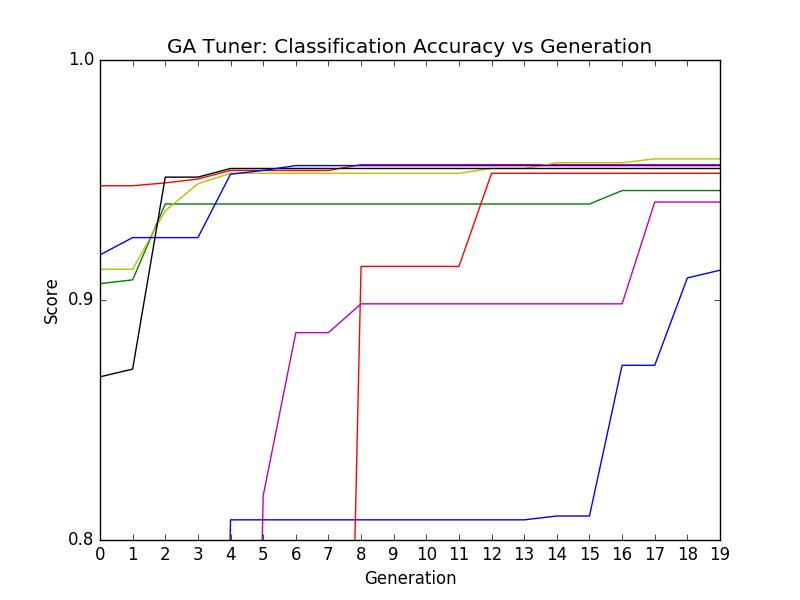
\includegraphics[width=\linewidth]{sections/imgs/ga/summary.png}
	    \caption{Convergence process of GA tuning}
	    \label{fig:ga_tuning_summary}
	\end{subfigure}
	\begin{subfigure}[b]{0.45\linewidth}
		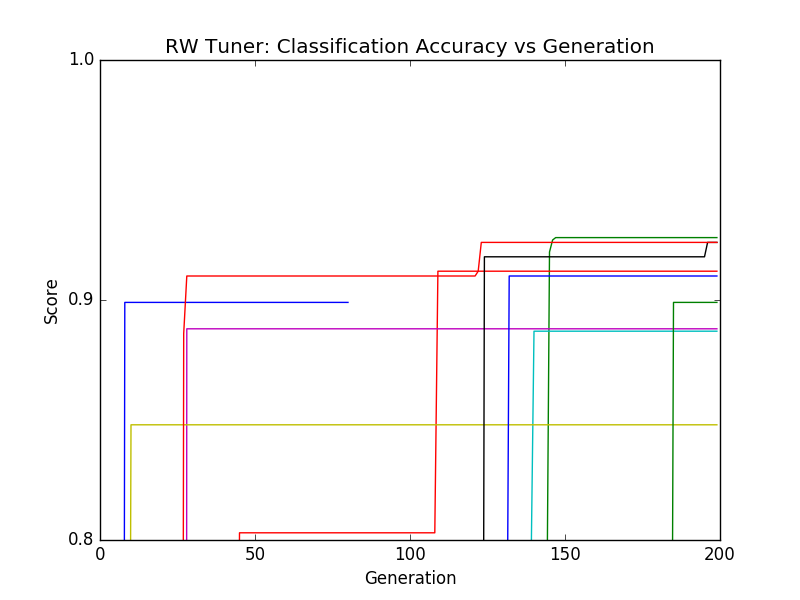
\includegraphics[width=\linewidth]{sections/imgs/random_walk/summary.png}
		\caption{Convergence process of Random Walk tuning}
		\label{fig:rw_tuning_summary}
	\end{subfigure}
	
	\begin{subfigure}[b]{0.45\linewidth}
		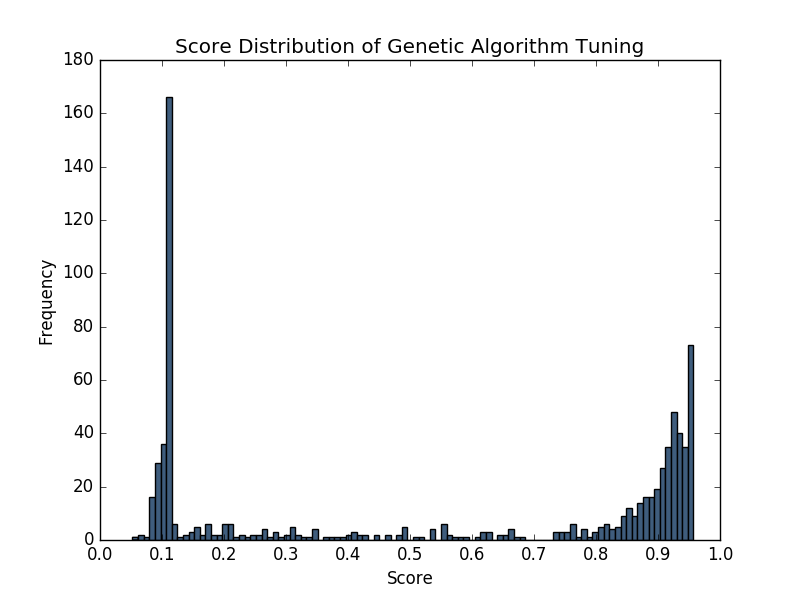
\includegraphics[width=\linewidth]{sections/imgs/ga/score_distribution.png}
		\caption{Accuracy of models tuned by GA}
		\label{fig:ga_tuning_score_distribution}
	\end{subfigure}
	\begin{subfigure}[b]{0.45\linewidth}
		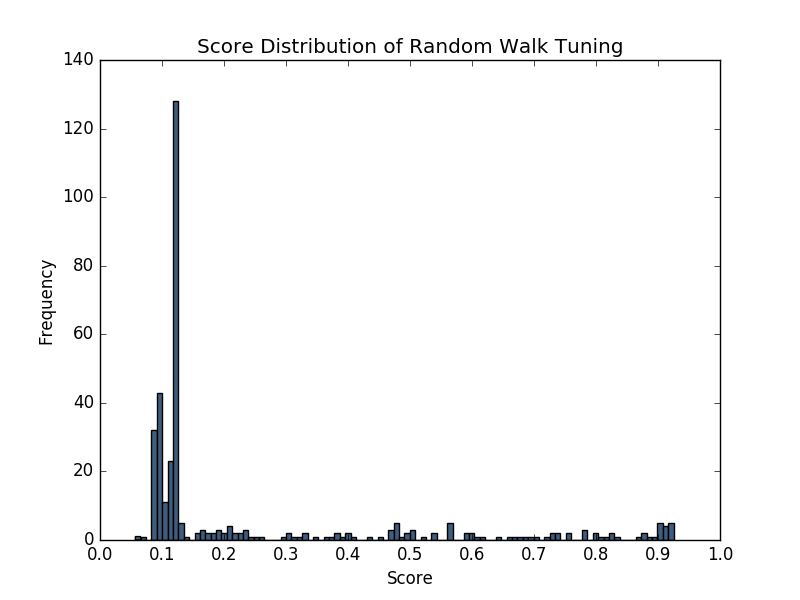
\includegraphics[width=\linewidth]{sections/imgs/random_walk/score_distribution.png}
		\caption{Accuracy of models tuned by Random Walk}
		\label{fig:rw_tuning_score_distribution}
	\end{subfigure}
	\caption{Preliminary Experiment Results}
	\label{fig:prelim_results}
\end{figure}

The experiment was executed 10 times with different random seeds for each run, where both GA and RW ran on the same set of random seeds for a fair comparison. The results, 8 out of 10 GA runs produced good feed-forward hyperparameters capable of scoring $> 80\%$ accuracy (see Fig~\ref{fig:ga_tuning_summary}). RW on the other hand has 10 out of 10 runs as seen in Fig~\ref{fig:rw_tuning_summary} (with one question able data point; the blue run which halted at around $80^{\text{th}}$ generation). 

At first glance it may appear that RW is better than GA based purely on convergence sucess rates (10 out of 10 as supposed to 8 with GA), however looking closer at the quality of the results, out of 8 of the GA runs, all of them score $90\%$ and above where as RW only has 5 out of 10. 

This leads us to conclude that despite only 10\% of the MNIST dataset was used, successful GA runs discovers higher quality solutions compared to exploring the hyperparameter space by random. This can be confirmed with the score distributions of both approaches. The results discussed gave us some confidence that the use of GA to tune hyperparameters might be helpful for this project.



\subsubsection{Experiments and Results with the Right Whale Data}
\label{sec:ga_cnn_tuner}
After our preliminary success with the MNIST dataset, we decided to use the GA tuner on the Right Whale dataset $D_{2}$ and $D_{3}$, only 50\% of both train and test dataset were used due to time constraints, evaluating a single network can take between 1 to 6 hours depending on network size and parameters. The experimental setup is very similar to the preliminary experiments, however instead of evolving hyperparamters for a feed-forward neural network, we are now evolving hyperparamters for a CNN. 

The hyperparameters the GA is tuning includes the number of convolutional layers, number of filters for each convolutional layer, activation functions on each convolutional layer, etc, for more details on what hyperparameters were tuned please see supplementary material~\ref{sup:cnn_hyperparameters}. For the GA tuner's own hyperparameters we have set the population size to 10, tournament selection of size 2, mutation and crossover probability at 20\% and 50\% respectively, with the mutation percentage set at 10\% of the chromosome. Below are our best results of the GA CNN tuner on $D_{2}$ and $D_{3}$:

\begin{wrapfigure}{L}[0pt]{0.45\textwidth}
	\vspace{-0.5cm}
	
	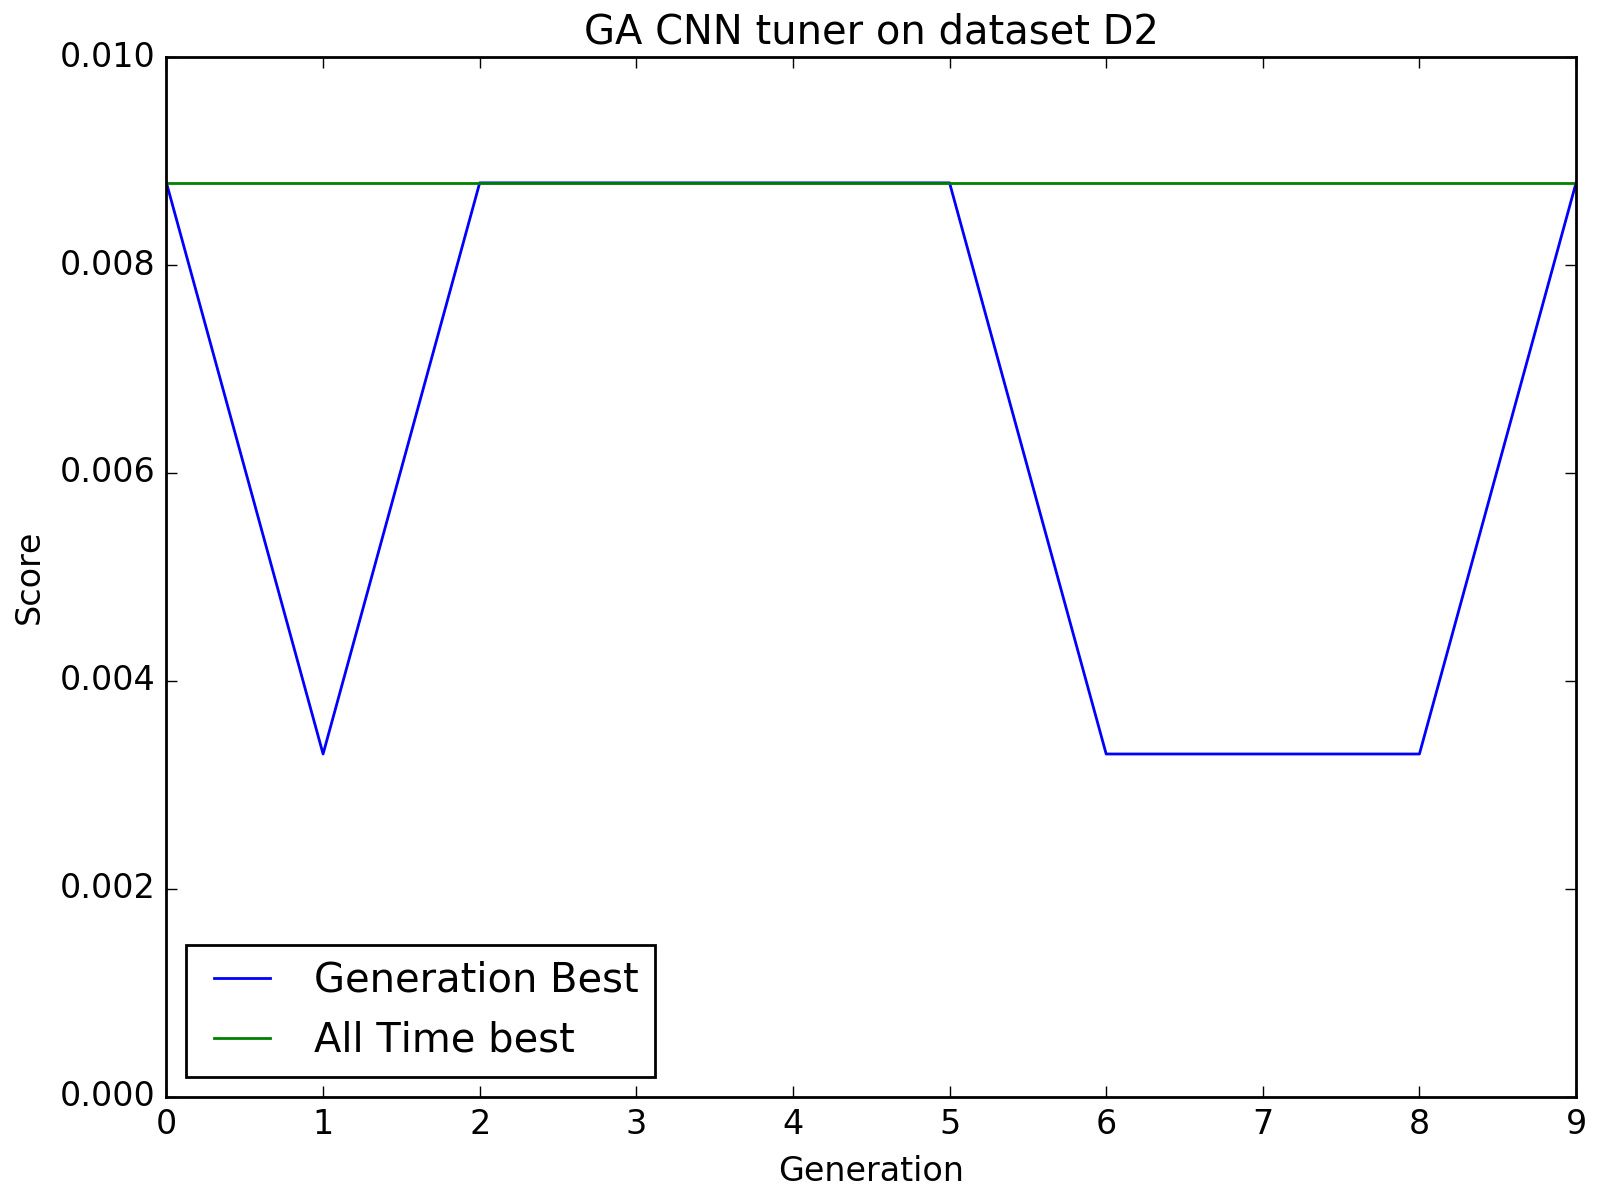
\includegraphics[width=\linewidth]{sections/imgs/ga/ga_cnn_tuner-dataset_2.png}
	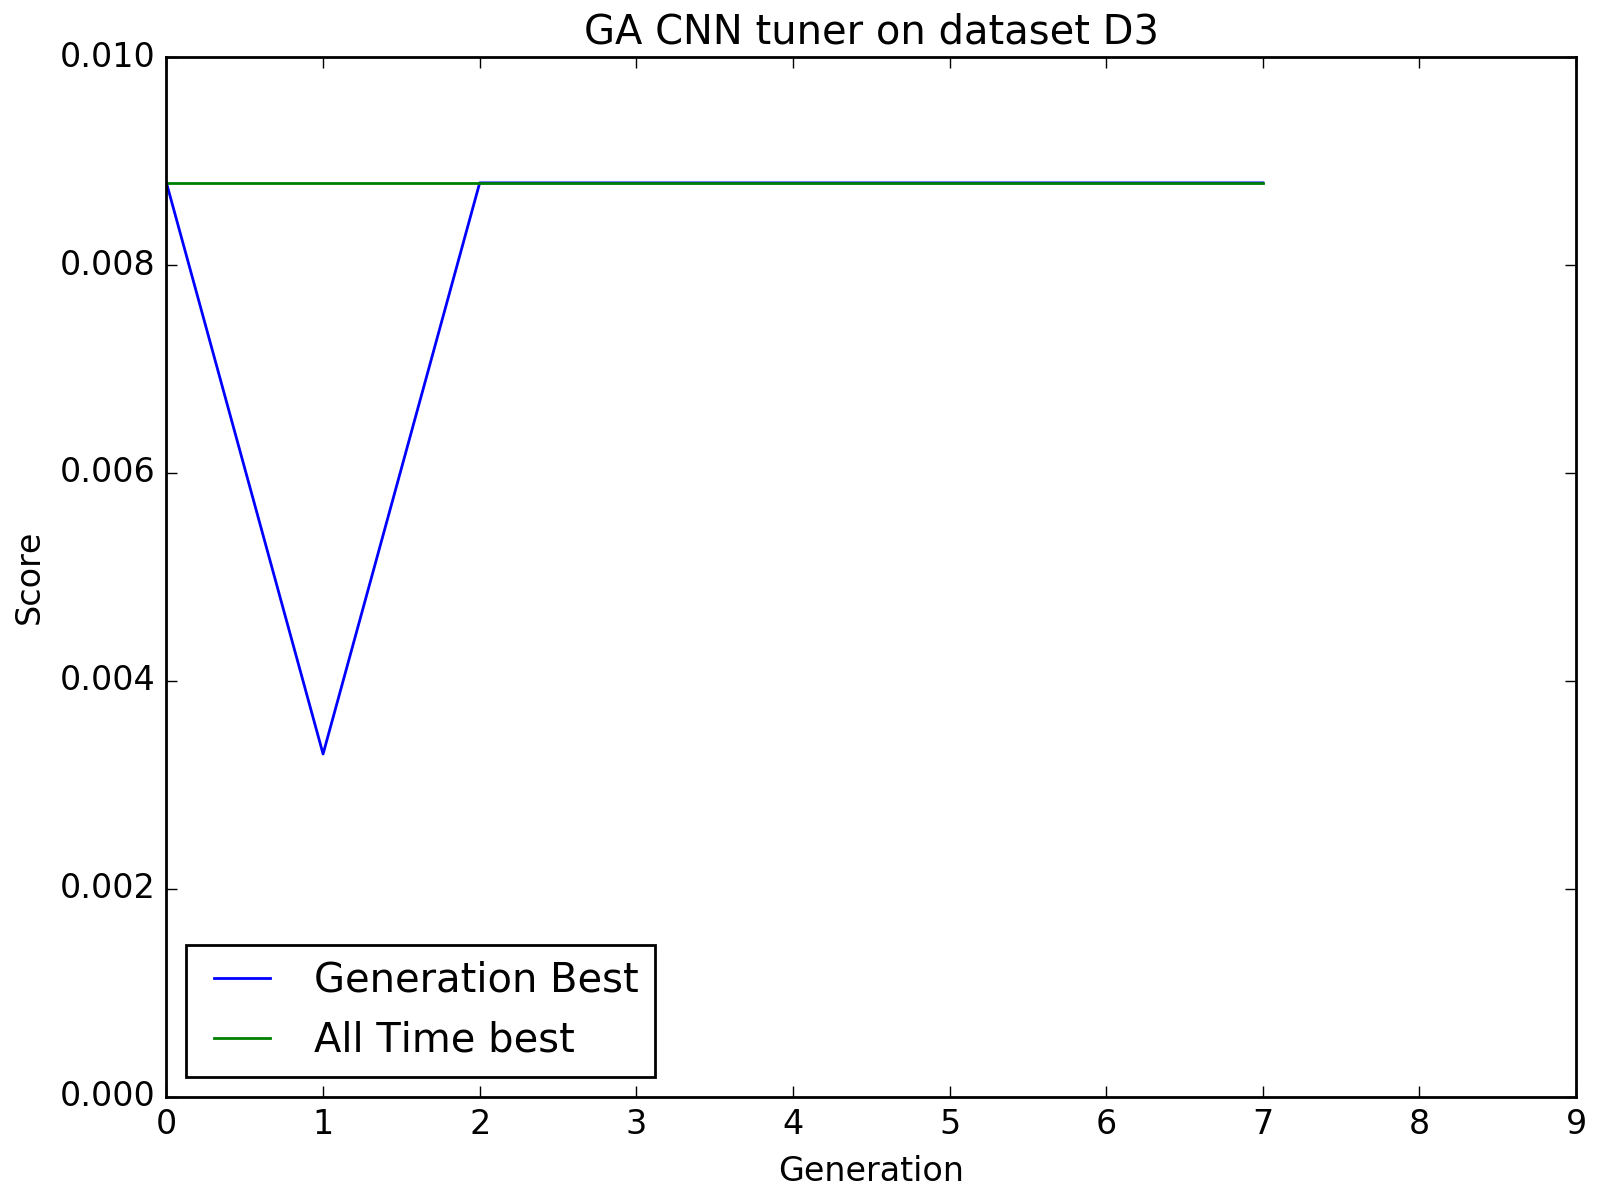
\includegraphics[width=\linewidth]{sections/imgs/ga/ga_cnn_tuner-dataset_3.png}
	
	\caption{GA CNN Tuner Results on D2 and D3}
	\label{fig:ga_cnn_results}
\end{wrapfigure}

From Figure~\ref{fig:ga_cnn_results} we can observed the results for the GA CNN tuner for both datasets performed very poorly, with the best classification accuracy of approximately 0.86\%. There are many possible reasons why the results produced were so poor, the first being that only 50\% of $D_{2}$ and $D_{3}$ were used could have had a major impact on convergence of the neural network, considering the data itself is already quite sparse. Secondly the population size of which the GA is tuning with is too small, usually GA experiements require a population size of atleast 50 and above to obtain a good sample of the search space. Lastly, more generations of the GA should have been performed to see if GA will eventually converge. 

Correcting these known failures however was impractical for the time we had,  considering if we increased the dataset size trained/tested to 100\%, and allow the GA to run more generations, it could take a week or more to finish 1 GA tuning run. We lacked the time and resources to do that. Additionally we faced some implementation problems with regards to Keras, during training of a network generated by the GA, the execution would suddenely halt and exit with "Floating Point Exception" with no other error messages, we found this very pecuilar considering we antissipated that error and have already encapsulated the code with a try and catch of all exception types. That is why the GA CNN tuner on dataset $D_{3}$ stopped earlier than generation 9 (see Figure~\ref{fig:ga_cnn_results} and Supplementary Material~\ref{sup:ga_cnn_tuner_eval_func})





